%!TEX root = ../../Heun_Dale_Haney_A_dynamic_approach_to_input_output_modeling.tex
%%%%%%%%%%%%%%%%%%%%% chapter.tex %%%%%%%%%%%%%%%%%%%%%%%%%%%%%%%%%
%
% sample chapter
%
% Use this file as a template for your own input.
%
%%%%%%%%%%%%%%%%%%%%%%%% Springer-Verlag %%%%%%%%%%%%%%%%%%%%%%%%%%
%\motto{Use the template \emph{chapter.tex} to style the various elements of your chapter content.}

%%%%%%%%%%%%%%%%%%%%%%%%%%%%%%%%%%%%%%
%%%%%%%%%% Energy Intensity %%%%%%%%%%
%%%%%%%%%%%%%%%%%%%%%%%%%%%%%%%&&&&%%%
\chapter{Energy intensity}
% Always give a unique label
\label{chap:intensity} 
% use \chaptermark{} to alter or adjust the chapter heading in the running head
\chaptermark{intensity}
%%%%%%%%%%%%%%%%%%%%%%%%%%%%%%%%%%
%%%%%%%%%%%%%%%%%%%%%%%%%%%%%%%%%%
%%%%%%%%%%%%%%%%%%%%%%%%%%%%%%%%%%

\abstract*{[NEED TO ADD ABSTRACT HERE]}

%% \abstract{Each chapter should be preceded by an abstract (10--15 lines long) that summarizes the content. The abstract will appear \textit{online} at \url{www.SpringerLink.com} and be available with unrestricted access. This allows unregistered users to read the abstract as a teaser for the complete chapter. As a general rule the abstracts will not appear in the printed version of your book unless it is the style of your particular book or that of the series to which your book belongs.\newline\indent
%% Please use the 'starred' version of the new Springer \texttt{abstract} command for typesetting the text of the online abstracts (cf. source file of this chapter template \texttt{abstract}) and include them with the source files of your manuscript. Use the plain \texttt{abstract} command if the abstract is also to appear in the printed version of the book.}

%% Use the template \emph{chapter.tex} together with the Springer document class SVMono (monograph-type books) or SVMult (edited books) to style the various elements of your chapter content in the Springer layout.


In Chapters~\ref{chap:direct_energy},~\ref{chap:embodied_energy}, and~\ref{chap:value}, 
we defined flows of direct energy, embodied energy, and value in an economy.
In this chapter, we merge energy and value together to estimate
the energy intensity of economic sectors.


%%%%%%%%%% Methodology %%%%%%%%%%
\section{Methodology}
%%%%%%%%%%

Energy intensity ($\varepsilon$)\nomenclature[e]{$\varepsilon$}{energy intensity [J/\$]}
is the ratio 
of total energy ($\dot{T}$) 
and value ($\dot{X}$) outflow rates 
from an economic sector, 
such that for the $j^{\mathrm{th}}$ goods and services sector,

\begin{equation} \label{eq:epsilon_output_def_g_and_s}
	\varepsilon_{j} \equiv \frac{\dot{T}_{j}}{\dot{X}_{j}},
\end{equation} 

\noindent{}and $\varepsilon$ is in units of J/\$. 
For inter-sector flows, we have

\begin{equation} \label{eq:epsilon_transfers_1}
	\varepsilon_{jk} = \frac{\dot{T}_{jk}}{\dot{X}_{jk}}.
\end{equation}

Furthermore, we note that 

\begin{equation} \label{eq:epsilon_equiv_1}
	\varepsilon_{j} = \varepsilon_{jk}
\end{equation}

\noindent{}for all $k$, because the energy intensity 
of sector $j$'s output is independent of its destination ($k$). 
I.e., we assume that all goods produced by a sector 
are produced at the average energy intensity 
of that sector.\footnote{If this approach is unsatisfactory, 
the sector may be divided into sub-sectors 
with different energy intensities.}

We define the input-ouput ratio ($a_{ij}$)\nomenclature[a]{$a$}{input-output ratio [-]}
that represents the input 
of good $i$ required to produce a unit of output from sector $j$.

\begin{equation} \label{eq:aij_def}
	a_{ij} \equiv \frac{\dot{X}_{ij}}{\dot{X}_{j}}
\end{equation}

Input-output ratios are given in mixed units, 
depending on both the purpose of each sector of the economy 
and the type of input as shown in Figure~\ref{fig:A_matrix_units}.

\begin{figure}[h!]
\centering\
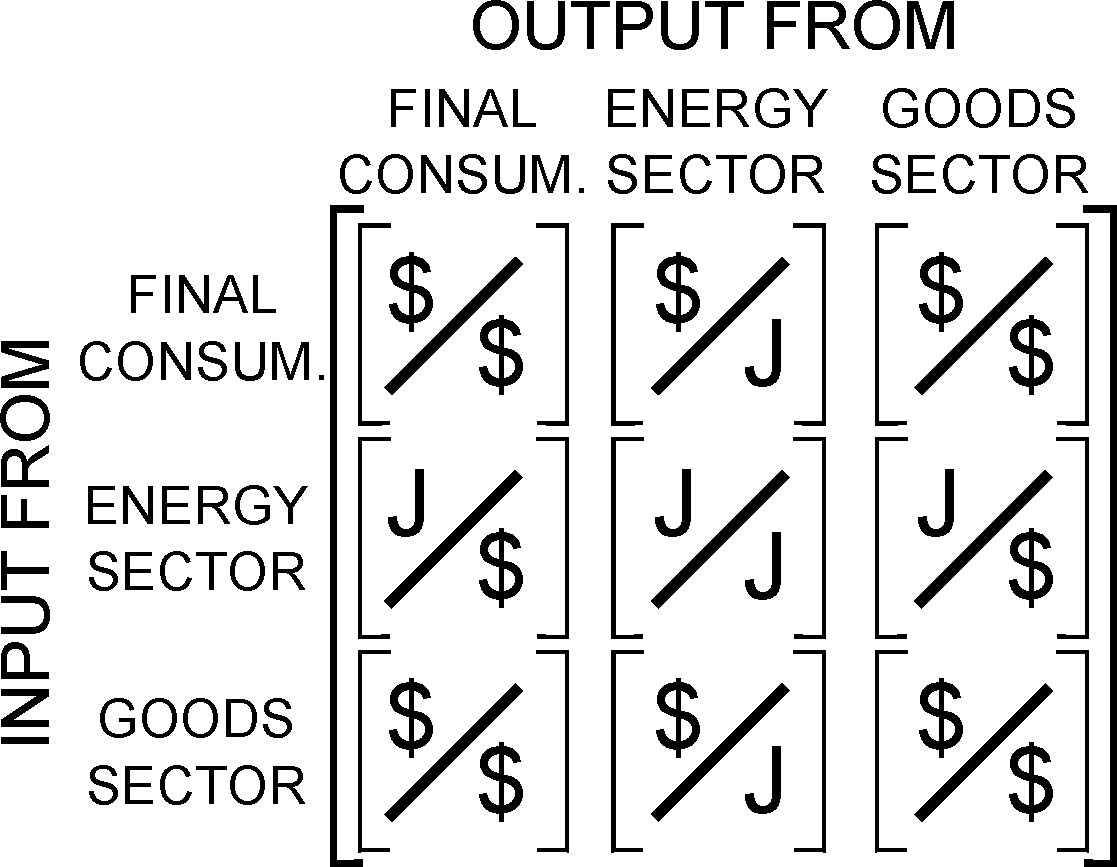
\includegraphics[width=0.4\linewidth]{Part_2/Chapter_Intensity/images/I-O_units.pdf}
\caption{Units for input-output ratios ($a$). **** Mik: Can we turn this
into a matrix where row zero and column zero represent society, 
row and column 1 represents energy, and the rest represent goods and services? ****}
\label{fig:A_matrix_units}
\end{figure}


%%%%%%%%%% Example A %%%%%%%%%%
\section{Example A: single-sector economy} % chktex 13
%%%%%%%%%%

With reference to Figures~\ref{fig:A_energy}, 
\ref{fig:A_total_energy_T_dot}, 
and~\ref{fig:A_value},
the energy intensity ($\varepsilon_{1}$) of a single-sector economy is calculated by

\begin{equation} \label{eq:A-energy_intensity}
	\varepsilon_{1} 
	= \frac{\dot{T}_{1}}{\dot{X}_{1}} 
	= \frac{\dot{T}_{11}}{\dot{X}_{11}}.
\end{equation}

Appendix~\ref{chap:infinite_series} illustrates that the energy 
intensity of a single-sector economy ($\varepsilon_{1}$) 
is comprised of the sum of the infinite recursions
of energy consumed during production of output ($\dot{X}_{1}$).

To estimate energy intensities
when more than one economic sector is involved, 
we move to Examples~B and~C in the following sections.


%%%%%%%%%% Example B %%%%%%%%%%
\section{Example B: two-sector economy} % chktex 13
%%%%%%%%%%

With reference to Figures~\ref{fig:B_energy}, 
\ref{fig:B_total_energy},
and~\ref{fig:B_value}, 
the energy intensity ($\varepsilon_{2}$) 
of the production sector is given by

\begin{equation} \label{eq:single_sector_energy_intensity}
	\varepsilon_{2} 
	= \frac{\dot{T}_{2}}{\dot{X}_{2}} 
	= \frac{\dot{T}_{22}}{\dot{X}_{22}}.
\end{equation}

\noindent{}Thus,

\begin{equation} \label{eq:T_dot_1_single_sector}
	\dot{T}_{2} = \varepsilon_{2}\dot{X}_{2},
\end{equation}

The input-output ratio 
for the production sector's self-use of output ($a_{22}$) is

\begin{equation} \label{eq:io_ratio_single_sector}
	a_{22} = \frac{\dot{X}_{22}}{\dot{X}_{2}},
\end{equation}

\noindent{}thus

\begin{equation} \label{eq:T_dot_11_single_sector}
	\dot{T}_{22} = \varepsilon_{2}a_{22}\dot{X}_{2}.
\end{equation}

Realizing that 
(a) $\frac{\mathrm{d}T_2}{\mathrm{d}t} = \frac{\mathrm{d}B_2}{\mathrm{d}t}$ 
due to $\frac{\mathrm{d}E_2}{\mathrm{d}t} = 0$, because direct energy
does not accumulate within economic sectors and
(b) $\dot{T}_{02} = \dot{E}_{02}$ due to $\dot{B}_{02} = 0$, 
because embodied energy appears only in the \emph{output} of a sector, and
substituting Equations~\ref{eq:T_dot_1_single_sector} 
and~\ref{eq:T_dot_11_single_sector} into Equation~\ref{eq:CV_T_2} gives

\begin{equation} \label{eq:dB1/dt_single_sector_after_substituting_eps_and_a}
	\frac{\mathrm{d}B_{2}}{\mathrm{d}t} 
	= \dot{E}_{02} 
	+ \dot{T}_{12}
	+ \varepsilon_{2}a_{22}\dot{X}_{2} 
	- \varepsilon_{2}\dot{X}_{2} 
	- \gamma_{2}B_{2}.
\end{equation}

To extend Equation~\ref{eq:dB1/dt_single_sector_after_substituting_eps_and_a}
to a matrix formulation, we turn to Example~C.


%%%%%%%%%% Example C %%%%%%%%%%
\section{Example~C: three-sector economy} % chktex 13
\label{sec:C-intensity}
%%%%%%%%%%

The three-sector economy of Example~C affords the opportunity 
to develop a matrix version 
of the total energy accounting equation (\ref{eq:C-CV_T_123})
and to develop an equation that estimates the
energy intensity of economic sectors. 
We begin with a matrix version of the total energy accounting equation.


%+++++++++ Example C: Total energy equation ++++++++++
\subsection{Total energy accounting equation}
%+++++++++

We apply Equation~\ref{eq:C-CV_T_123} to the three-sector
economy shown in 
Figures~\ref{fig:C_energy},~\ref{fig:C_total_energy}, and~\ref{fig:C_value}
to obtain the following total energy accounting equations
for the Energy~(2) and Goods and Services~(3) sectors 
of the three-sector economy:

\begin{equation} \label{eq:C-Total_Energy_Sec_2-a}
	\frac{\mathrm{d}T_{2}}{\mathrm{d}t} 
	= \dot{T}_{02}  
	+ \dot{T}_{12}
	+ \dot{T}_{22}
	+ \dot{T}_{32}
	- \dot{T}_{2}
	- \dot{T}_{20}
\end{equation}

\noindent{}and

\begin{equation} \label{eq:C-Total_Energy_Sec_3-a}
	\frac{\mathrm{d}T_{3}}{\mathrm{d}t} 
	= \dot{T}_{03}  
	+ \dot{T}_{13}
	+ \dot{T}_{23}
	+ \dot{T}_{33}
	- \dot{T}_{3}
	- \dot{T}_{30}.
\end{equation}

\noindent{}Similar to Example~B, we realize that 
(a) $\frac{\mathrm{d}T_i}{\mathrm{d}t} = \frac{\mathrm{d}B_i}{\mathrm{d}t}$ 
due to $\frac{\mathrm{d}E_i}{\mathrm{d}t} = 0$, because direct energy
does not accumulate within economic sectors and
(b) $\dot{T}_{0j} = \dot{E}_{0j}$ due to $\dot{B}_{0j}~=~0$, 
because embodied energy appears only in the \emph{output} of a sector, and
we substitute $\dot{T}_{j} = \varepsilon_{j} \dot{X}_{j}$ 
and $\dot{T}_{jk} = \varepsilon_{j} \dot{X}_{jk}$ 
into Equations~\ref{eq:C-Total_Energy_Sec_2-a}
and~\ref{eq:C-Total_Energy_Sec_3-a} to obtain

\begin{equation} \label{eq:C-Total_Energy_Sec_2-b}
	\frac{\mathrm{d}B_{2}}{\mathrm{d}t}
	= \dot{E}_{02}
	+ \dot{T}_{12}
	+ \varepsilon_{2} \dot{X}_{22}
	+ \varepsilon_{3} \dot{X}_{32}
	- \varepsilon_{2} \dot{X}_{2}
	- \gamma_{2} B_{2}
\end{equation}

\noindent{}and

\begin{equation} \label{eq:C-Total_Energy_Sec_3-b}
	\frac{\mathrm{d}B_{3}}{\mathrm{d}t}
	= \dot{E}_{03}
	+ \dot{T}_{13}
	+ \varepsilon_{2} \dot{X}_{23}
	+ \varepsilon_{3} \dot{X}_{33}
	- \varepsilon_{3} \dot{X}_{3}
	- \gamma_{3} B_{3}.
\end{equation}


%%%%%%%%%% Example C: Matrix formulation %%%%%%%%%%
\subsection{Matrix formulation} % chktex 13
\label{sec:C-matrix}
%%%%%%%%%%

\noindent{}Equations~\ref{eq:C-Total_Energy_Sec_2-b} 
and~\ref{eq:C-Total_Energy_Sec_3-b} can be rewritten 
in matrix notation as

\begin{equation} \label{eq:C-Expanded_Matrix_Form}
	\begin{split}
		\begin{Bmatrix}
			\frac{\mathrm{d}B_{2}}{\mathrm{d}t} \\[0.4em] % Adds some vertical space.
			\frac{\mathrm{d}B_{3}}{\mathrm{d}t} 
		\end{Bmatrix}
		=
		\begin{Bmatrix}
			\dot{E}_{02}\\
			\dot{E}_{03}
		\end{Bmatrix}
		& +                                               % & sets alighment tab
		\begin{Bmatrix}
			\dot{T}_{12}\\
			\dot{T}_{13}
		\end{Bmatrix}
		+
		\begin{bmatrix}
			\dot{X}_{22} & \dot{X}_{32}\\
			\dot{X}_{23} & \dot{X}_{33}
		\end{bmatrix}
		\begin{Bmatrix}
			\varepsilon_{2}\\
			\varepsilon_{3}
		\end{Bmatrix} \\                                  % \\ gives line break
		& -                                               % & aligns to previous tab
		\begin{bmatrix}
			\dot{X}_{2} & 0          \\
			0           & \dot{X}_{3}
		\end{bmatrix}
		\begin{Bmatrix}
			\varepsilon_{2}\\
			\varepsilon_{3}
		\end{Bmatrix}
		-
		\begin{bmatrix}
			\gamma_{2} & 0          \\
			0          & \gamma_{3}
		\end{bmatrix}
		\begin{Bmatrix}
			B_{2}\\
			B_{3}
		\end{Bmatrix}		
	\end{split}
\end{equation}

\noindent{}If we define the following matrices and vectors:

\begin{equation} \label{eq:dBdt_vec_def}
	\frac{\mathrm{d}\vec{B}}{\mathrm{d}t} 
	\equiv
	\begin{Bmatrix}	
		\frac{\mathrm{d}B_{2}}{\mathrm{d}t}	\\[0.4em] % Adds some vertical space.
		\frac{\mathrm{d}B_{3}}{\mathrm{d}t}
	\end{Bmatrix},
\end{equation}

\begin{equation} \label{eq:E_vec_def}
	\vec{E}_{0} 
	\equiv
	\begin{Bmatrix}
		\dot{E}_{02} \\
		\dot{E}_{03}
	\end{Bmatrix},\nomenclature[E]{$\vec{E}_{0}$}{vector of direct energy inputs 
													from the biosphere [W]}
\end{equation}

\begin{equation} \label{eq:T_vec_def}
	\vec{T}_{1} 
	\equiv
	\begin{Bmatrix}
		\dot{T}_{12} \\
		\dot{T}_{13}
	\end{Bmatrix},\nomenclature[T]{$\vec{T}_{1}$}{vector of total energy inputs 
													from society to the economy [W]}
\end{equation}

\begin{equation} \label{eq:X_t_matrix_def}
	\vec{X}_{t} 
	\equiv
	\begin{bmatrix}
		\dot{X}_{22} & \dot{X}_{23} \\
		\dot{X}_{32} & \dot{X}_{33}
	\end{bmatrix},\nomenclature[X]{$\vec{X}_{t}$}{transaction matrix [\$/year]}
\end{equation}

\begin{equation} \label{eq:eps_vec_def}
	\bm{\varepsilon} 
	\equiv
	\begin{Bmatrix}
		\varepsilon_{2}	\\
		\varepsilon_{3}
	\end{Bmatrix},\nomenclature[e]{$\bm{\varepsilon}$}{column vector 
														of sector energy intensities [J/\$]}
\end{equation}

\begin{equation} \label{eq:X_hat_matrix_def}
	\hat{\vec{X}} 
	\equiv
	\delta_{ij} \dot{X}_{j} 
	= 
	\begin{bmatrix}
		\dot{X}_{2}		&	0	  \\
		0				&	\dot{X}_{3}	\\
	\end{bmatrix},\nomenclature[X]{$\hat{\vec{X}}$}{matrix of sector outputs [\$/year]}
\end{equation}

\begin{equation} \label{eq:gamma_hat_matrix_def}
	\hat{\bm{\gamma}}
	\equiv
	\delta_{ij} \gamma_{j}
	=
	\begin{bmatrix}
		\gamma_{2} & 0         \\
		0          & \gamma_{3}
	\end{bmatrix},
\end{equation}\nomenclature[g]{$\hat{\bm{\gamma}}$}{matrix of depreciation rates [\$/year]}

\noindent{}and

\begin{equation} \label{eq:B_vec_def}
	\vec{B} 
	\equiv
	\begin{Bmatrix}	
		B_{2} \\
		B_{3}
	\end{Bmatrix};
\end{equation}

\noindent{}with the ``Kronecker delta''

\begin{equation}\label{eq:k_delta}
	\delta_{ij} 
	=
	\begin{cases}	
		0	&	\text{if  } i \neq j	\\
		1 	& 	\text{if  } i = j
	\end{cases};
\end{equation}\nomenclature[d]{$\delta_{ij}$}{Kronecker delta}

\noindent{}we can rewrite Equation~\ref{eq:C-Expanded_Matrix_Form}
compactly as

\begin{equation} \label{eq:matrix_leontief_pre_1}
	\frac{\mathrm{d}\vec{B}}{\mathrm{d}t} 
	= \vec{E}_{0}
	+ \vec{T}_{1}
	+ \vec{X}_{t}^{\mathrm{T}}\bm{\varepsilon} 
	- \hat{\vec{X}}\bm{\varepsilon}
	- \hat{\bm{\gamma}}\vec{B}.
\end{equation}

\noindent{}Equation~\ref{eq:matrix_leontief_pre_1} can be simplified to

\begin{equation} \label{eq:matrix_leontief_pre_2}
	\frac{\mathrm{d}\vec{B}}{\mathrm{d}t} 
	= \vec{E}_{0}
	+ \vec{T}_{1}
	+ (\vec{X}_{t}^{\mathrm{T}} - \hat{\vec{X}})\bm{\varepsilon} 
	- \hat{\bm{\gamma}}\vec{B}.
\end{equation}

\noindent{}We can define the input-output matrix ($\vec{A}$) as

\begin{equation} \label{eq:A_matrix_def}
	\vec{A} 
	\equiv
	\begin{bmatrix}
		a_{22} & a_{23}	\\
		a_{32} & a_{33}	
	\end{bmatrix}.
\end{equation}\nomenclature[A]{$\vec{A}$}{input-output matrix [-]}

\noindent{}Appendix~\ref{app:Proof} shows that

\begin{equation} \label{eq:Xdifference1}
	\vec{X}_{t}^{\mathrm{T}} 
	- \hat{\vec{X}} 
	= \hat{\vec{X}} (\vec{A}^{\mathrm{T}} - \vec{I}),
\end{equation}

\noindent{}which allows Equation~\ref{eq:matrix_leontief_pre_2}
to be recast as

\begin{equation} \label{eq:matrix_leontief}
	\frac{\mathrm{d}\vec{B}}{\mathrm{d}t} 
	= \vec{E}_{0}
	+ \vec{T}_{1}
	+ \hat{\vec{X}} (\vec{A}^{\mathrm{T}} - \vec{I})\bm{\varepsilon} 
	- \hat{\bm{\gamma}}\vec{B}.
\end{equation}

\noindent{}Equation~\ref{eq:matrix_leontief} is the matrix version 
of the total energy accounting equation
written in terms of energy intensities ($\bm{\varepsilon}$)
and input-output ratios ($\vec{A}$).
Equation~\ref{eq:C-Expanded_Matrix_Form} applies 
for the three-sector economy of Example~C, 
but the equivalent matrix formulation (Equation~\ref{eq:matrix_leontief}) 
can be extended to any desired level 
of economic and energy sector disaggregation 
by expanding the vectors and matrices in 
Equations~\ref{eq:dBdt_vec_def}--\ref{eq:B_vec_def}
and~\ref{eq:A_matrix_def} to include
all sectors of the economy.~\cite{Casler1984,Bullard:1978vd}

Equation~\ref{eq:matrix_leontief} provides a means to 
estimate the embodied energy accumulation rate
in economic sectors $\left(\frac{\mathrm{d}\vec{B}}{\mathrm{d}t}\right)$ 
knowing only 
direct energy inputs to the economy from the biosphere ($\vec{E}_{0}$), 
total energy inputs from society to the economy ($\vec{T}_{1}$),
sector outputs ($\hat{\vec{X}}$), 
sector input-output ratios ($\vec{A}$), 
sector energy intensities ($\bm{\varepsilon}$), 
and sector physical depreciation rates ($\hat{\bm{\gamma}}\vec{B}$). 
In theory, the transaction matrix ($\vec{X}_{t}$) is not required 
if the input-ouput matrix ($\vec{A}$) is known, 
though in practice, 
knowledge of input-output matrix ($\vec{A}$) 
would be derived from the transaction matrix ($\vec{X}_{t}$),
as shown in Appendix~\ref{chap:Estimating_A}.


%%%%%%%%%% Example C %%%%%%%%%%
\section{Estimating $\bm{\varepsilon}$}
%%%%%%%%%%

Equation~\ref{eq:matrix_leontief} can be rearranged to obtain

\begin{equation} \label{eq:epsilon_derivation_1}
	\hat{\vec{X}} (\vec{A}^{\mathrm{T}} - \vec{I}) \bm{\epsilon}
	= \frac{\mathrm{d}\vec{B}}{\mathrm{d}t}
	+ \hat{\bm{\gamma}} \vec{B}
	- \vec{E}_{0}
	- \vec{T}_{1} 
\end{equation}

\noindent{}and

\begin{equation} \label{eq:epsilon_derivation_2}
	\bm{\epsilon}
	= {\left[ \hat{\vec{X}} (\vec{A}^{\mathrm{T}} - \vec{I}) \right]}^{-1}
		\left[
			\frac{\mathrm{d}\vec{B}}{\mathrm{d}t}
			+ \hat{\bm{\gamma}} \vec{B}
			- \vec{E}_{0}
			- \vec{T}_{1} 
		\right].
\end{equation}

\noindent{}We apply the matrix identity~\cite[Formula 6.2, p. 308]{Beyer:1991vd}

\begin{equation} \label{eq:matrix_identity_Beyer}
	{\left(\vec{A}\vec{B}\vec{C}\right)}^{-1} 
	= \vec{C}^{-1} \vec{B}^{-1} \vec{A}^{-1}
\end{equation}

\noindent{}to the right side of Equation~\ref{eq:epsilon_derivation_2} to obtain

\begin{equation} \label{eq:epsilon_derivation_3}
	\bm{\epsilon}
	= {(\vec{A}^{\mathrm{T}} - \vec{I})}^{-1} {\hat{\vec{X}}}^{-1} 
		\left[
			\frac{\mathrm{d}\vec{B}}{\mathrm{d}t}
			+ \hat{\bm{\gamma}} \vec{B}
			- \vec{E}_{0}
			- \vec{T}_{1} 
		\right].
\end{equation}

\noindent{}Changing signs on the right side 
of Equation~\ref{eq:epsilon_derivation_2} gives

\begin{equation} \label{eq:epsilon_leontief_with_A}
	\bm{\varepsilon} 
	= {(\vec{I} - \vec{A}^{\mathrm{T}})}^{-1}\hat{\vec{X}}^{-1}
		\left[\vec{E}_{0} 
				+ \vec{T}_{1} 
				- \frac{\mathrm{d}\vec{B}}{\mathrm{d}t} 
				- \hat{\bm{\gamma}}\vec{B}
		\right].
\end{equation}

\noindent{}Equation~\ref{eq:epsilon_leontief_with_A} allows estimation 
of the energy intensity 
of economic sectors ($\bm{\varepsilon}$) 
knowing only 
sector input-output ratios ($\vec{A}$), 
sector outputs ($\hat{\vec{X}}$), 
energy input to the economy from the biosphere~($\vec{E}_{0}$), 
total energy input from society to the economy~($\vec{T}_{1}$),
sector embodied energy accumulation rates~$\left(\frac{\mathrm{d}\vec{B}}{\mathrm{d}t}\right)$,
and sector physical depreciation rates~($\hat{\bm{\gamma}}\vec{B}$).

Again, the transaction matrix ($\vec{X}_{t}$) is not required 
for estimating the energy intensity of economic sectors ($\bm{\varepsilon}$)
if the input-ouput matrix ($\vec{A}$) is known, 
though in practice, 
knowledge of input-output matrix ($\vec{A}$) 
would be derived from the transaction matrix ($\vec{X}_{t}$),
as shown in Appendix~\ref{chap:Estimating_A}.


%%%%%%%%%% Intensity: Auto industry example %%%%%%%%%%
\section{Energy intensity of the auto industry}
\label{sec:intensity_auto}
%%%%%%%%%%

***** Becky complete this section. Is there anything to include here? *****

%%%%%%%%%% Intensity: Summary %%%%%%%%%%
\section{Summary}
\label{sec:intensity_summary}
%%%%%%%%%%





\bibliographystyle{unsrt}
\bibliography{../../EROI_review_v2}


% Always give a unique label
% and use \ref{<label>} for cross-references
% and \cite{<label>} for bibliographic references
% use \sectionmark{}
% to alter or adjust the section heading in the running head
%% Instead of simply listing headings of different levels we recommend to let every heading be followed by at least a short passage of text. Furtheron please use the \LaTeX\ automatism for all your cross-references and citations.

%% Please note that the first line of text that follows a heading is not indented, whereas the first lines of all sequent paragraphs are.

%% Use the standard \verb|equation| environment to typeset your equations, e.g.
%
%% \begin{equation}
%% a \times b = c\;,
%% \end{equation}
%
%% however, for multiline equations we recommend to use the \verb|eqnarray|
%% environment\footnote{In physics texts please activate the class option \texttt{vecphys} to depict your vectors in \textbf{\itshape boldface-italic} type - as is customary for a wide range of physical jects.}.
%% \begin{eqnarray}
%% a \times b = c \nonumber\\
%% \vec{a} \cdot \vec{b}=\vec{c}
%% \label{eq:01}
%% \end{eqnarray}

%% \section{section Heading}
%% \label{sec:2}
%% Instead of simply listing headings of different levels we recommend to let every heading be followed by at least a short passage of text. Furtheron please use the \LaTeX\ automatism for all your cross-references\index{cross-references} and citations\index{citations} as has already been described in Sect.~\ref{sec:2}.

%% \begin{quotation}
%% Please do not use quotation marks when quoting texts! Simply use the \verb|quotation| environment -- it will automatically render Springer's preferred layout.
%% \end{quotation}


%% \section{section Heading}
%% Instead of simply listing headings of different levels we recommend to let every heading be followed by at least a short passage of text. Furtheron please use the \LaTeX\ automatism for all your cross-references and citations as has already been described in Sect.~\ref{sec:2}, see also Fig.~\ref{fig:1}\footnote{If you copy text passages, figures, or tables from other works, you must obtain \textit{permission} from the copyright holder (usually the original publisher). Please enclose the signed permission with the manucript. The sources\index{permission to print} must be acknowledged either in the captions, as footnotes or in a separate section of the book.}

%% Please note that the first line of text that follows a heading is not indented, whereas the first lines of all sequent paragraphs are.

% For figures use
%
%% \begin{figure}[b]
%% \sidecaption
% Use the relevant command for your figure-insertion program
% to insert the figure file.
% For example, with the option graphics use
%% \includegraphics[scale=.65]{figure}
%
% If not, use
%\picplace{5cm}{2cm} % Give the correct figure height and width in cm
%
%% \caption{If the width of the figure is less than 7.8 cm use the \texttt{sidecapion} command to flush the caption on the left side of the page. If the figure is positioned at the top of the page, align the sidecaption with the top of the figure -- to achieve this you simply need to use the optional argument \texttt{[t]} with the \texttt{sidecaption} command}
%% \label{fig:1}       % Give a unique label
%% \end{figure}


%% \paragraph{Paragraph Heading} %
%% Instead of simply listing headings of different levels we recommend to let every heading be followed by at least a short passage of text. Furtheron please use the \LaTeX\ automatism for all your cross-references and citations as has already been described in Sect.~\ref{sec:2}.

%% Please note that the first line of text that follows a heading is not indented, whereas the first lines of all sequent paragraphs are.

%% For typesetting numbered lists we recommend to use the \verb|enumerate| environment -- it will automatically render Springer's preferred layout.

%% \begin{enumerate}
%% \item{Livelihood and survival mobility are oftentimes coutcomes of uneven socioeconomic development.}
%% \begin{enumerate}
%% \item{Livelihood and survival mobility are oftentimes coutcomes of uneven socioeconomic development.}
%% \item{Livelihood and survival mobility are oftentimes coutcomes of uneven socioeconomic development.}
%% \end{enumerate}
%% \item{Livelihood and survival mobility are oftentimes coutcomes of uneven socioeconomic development.}
%% \end{enumerate}


%% \paragraph{paragraph Heading} In order to avoid simply listing headings of different levels we recommend to let every heading be followed by at least a short passage of text. Use the \LaTeX\ automatism for all your cross-references and citations as has already been described in Sect.~\ref{sec:2}, see also Fig.~\ref{fig:2}.

%% Please note that the first line of text that follows a heading is not indented, whereas the first lines of all sequent paragraphs are.

%% For unnumbered list we recommend to use the \verb|itemize| environment -- it will automatically render Springer's preferred layout.

%% \begin{itemize}
%% \item{Livelihood and survival mobility are oftentimes coutcomes of uneven socioeconomic development, cf. Table~\ref{tab:1}.}
%% \begin{itemize}
%% \item{Livelihood and survival mobility are oftentimes coutcomes of uneven socioeconomic development.}
%% \item{Livelihood and survival mobility are oftentimes coutcomes of uneven socioeconomic development.}
%% \end{itemize}
%% \item{Livelihood and survival mobility are oftentimes coutcomes of uneven socioeconomic development.}
%% \end{itemize}

%% \begin{figure}[t]
%% \sidecaption[t]
% Use the relevant command for your figure-insertion program
% to insert the figure file.
% For example, with the option graphics use
%% \includegraphics[scale=.65]{figure}
%
% If not, use
%\picplace{5cm}{2cm} % Give the correct figure height and width in cm
%
%% \caption{Please write your figure caption here}
%% \label{fig:2}       % Give a unique label
%% \end{figure}

%% \runinhead{Run-in Heading Boldface Version} Use the \LaTeX\ automatism for all your cross-references and citations as has already been described in Sect.~\ref{sec:2}.

%% \runinhead{Run-in Heading Italic Version} Use the \LaTeX\ automatism for all your cross-refer\-ences and citations as has already been described in Sect.~\ref{sec:2}\index{paragraph}.
% Use the \index{} command to code your index words
%
% For tables use
%
%% \begin{table}
%% \caption{Please write your table caption here}
%% \label{tab:1}       % Give a unique label
%
% For LaTeX tables use
%
%% \begin{tabular}{p{2cm}p{2.4cm}p{2cm}p{4.9cm}}
%% \hline\noalign{\smallskip}
%% Classes & class & Length & Action Mechanism  \\
%% \noalign{\smallskip}\svhline\noalign{\smallskip}
%% Translation & mRNA$^a$  & 22 (19--25) & Translation repression, mRNA cleavage\\
%% Translation & mRNA cleavage & 21 & mRNA cleavage\\
%% Translation & mRNA  & 21--22 & mRNA cleavage\\
%%Translation & mRNA  & 24--26 & Histone and DNA Modification\\
%%\noalign{\smallskip}\hline\noalign{\smallskip}
%%\end{tabular}
%%$^a$ Table foot note (with superscript)
%%\end{table}
%
%% \section{Section Heading}
%%\label{sec:3}
% Always give a unique label
% and use \ref{<label>} for cross-references
% and \cite{<label>} for bibliographic references
% use \sectionmark{}
% to alter or adjust the section heading in the running head
%% Instead of simply listing headings of different levels we recommend to let every heading be followed by at least a short passage of text. Furtheron please use the \LaTeX\ automatism for all your cross-references and citations as has already been described in Sect.~\ref{sec:2}.

%% Please note that the first line of text that follows a heading is not indented, whereas the first lines of all sequent paragraphs are.

%%If you want to list definitions or the like we recommend to use the Springer-enhanced \verb|description| environment -- it will automatically render Springer's preferred layout.

%%\begin{description}[Type 1]
%%\item[Type 1]{That addresses central themes pertainng to migration, health, and disease. In Sect.~\ref{sec:1}, Wilson discusses the role of human migration in infectious disease distributions and patterns.}
%%\item[Type 2]{That addresses central themes pertainng to migration, health, and disease. In Sect.~\ref{sec:2}, Wilson discusses the role of human migration in infectious disease distributions and patterns.}
%%\end{description}

%%\section{section Heading} %
%% In order to avoid simply listing headings of different levels we recommend to let every heading be followed by at least a short passage of text. Use the \LaTeX\ automatism for all your cross-references and citations citations as has already been described in Sect.~\ref{sec:2}.

%% Please note that the first line of text that follows a heading is not indented, whereas the first lines of all sequent paragraphs are.

%% \begin{svgraybox}
%% If you want to emphasize complete paragraphs of texts we recommend to use the newly defined Springer class option \verb|graybox| and the newly defined environment \verb|svgraybox|. This will produce a 15 percent screened box 'behind' your text.

%% If you want to emphasize complete paragraphs of texts we recommend to use the newly defined Springer class option and environment \verb|svgraybox|. This will produce a 15 percent screened box 'behind' your text.
%% \end{svgraybox}


%% \section{section Heading}
%%Instead of simply listing headings of different levels we recommend to let every heading be followed by at least a short passage of text. Furtheron please use the \LaTeX\ automatism for all your cross-references and citations as has already been described in Sect.~\ref{sec:2}.

%% Please note that the first line of text that follows a heading is not indented, whereas the first lines of all sequent paragraphs are.

%% \begin{theorem}
%% Theorem text goes here.
%% \end{theorem}
%
% or
%
%% \begin{definition}
%% Definition text goes here.
%% \end{definition}

%% \begin{proof}
%\smartqed
%% Proof text goes here.
%% \qed
%% \end{proof}

%%\paragraph{Paragraph Heading} %
%% Instead of simply listing headings of different levels we recommend to let every heading be followed by at least a short passage of text. Furtheron please use the \LaTeX\ automatism for all your cross-references and citations as has already been described in Sect.~\ref{sec:2}.

%% Note that the first line of text that follows a heading is not indented, whereas the first lines of all subsequent paragraphs are.
%
% For built-in environments use
%
%%\begin{theorem}
%%Theorem text goes here.
%%\end{theorem}
%
%%\begin{definition}
%%Definition text goes here.
%%\end{definition}
%
%%\begin{proof}
%%\smartqed
%% Proof text goes here.
%%\qed
%%\end{proof}
%
%% \begin{acknowledgement}
%% If you want to include acknowledgments of assistance and the like at the end of an individual chapter please use the \verb|acknowledgement| environment -- it will automatically render Springer's preferred layout.
%% \end{acknowledgement}
%
%% \section*{Appendix}
%% \addcontentsline{toc}{section}{Appendix}
%
%% When placed at the end of a chapter or contribution (as opposed to at the end of the book), the numbering of tables, figures, and equations in the appendix section continues on from that in the main text. Hence please \textit{do not} use the \verb|appendix| command when writing an appendix at the end of your chapter or contribution. If there is only one the appendix is designated ``Appendix'', or ``Appendix 1'', or ``Appendix 2'', etc. if there is more than one.

%% \begin{equation}
%% a \times b = c
%% \end{equation}
% Problems or Exercises should be sorted chapterwise
%% \section*{Problems}
%% \addcontentsline{toc}{section}{Problems}
%
% Use the following environment.
% Don't forget to label each problem;
% the label is needed for the solutions' environment
%% \begin{prob}
%% \label{prob1}
%% A given problem or Excercise is described here. The
%% problem is described here. The problem is described here.
%% \end{prob}

%% \begin{prob}
%% \label{prob2}
%% \textbf{Problem Heading}\\
%% (a) The first part of the problem is described here.\\
%% (b) The second part of the problem is described here.
%% \end{prob}


